\chapter{Empirische Evaluation}
\label{chap:evaluation}

Die Binärsuche von MULTIFIT ruft für jede getestete Kapazität $C$ ein Bin-Packing-Verfahren auf,
welches die Aufgaben in möglichst wenige Bins der Kapazität $C$ packt - in der Regel
approximativ -, und vergleicht die erreichte Binzahl mit $m$.
Die Suche selbst lässt sich deshalb mit jedem solchen Verfahren durchführen.
Die Gütegarantie aus Kapitel~\ref{chap:performanz} überträgt sich dabei jedoch nicht ohne
Weiteres: Sie beruht auf Implikation~\eqref{eq:ffd-akzeptiert}, welche für FFD formuliert und
bewiesen ist.
Dieses Kapitel misst in zwei getrennten Versuchsreihen, was der Austausch der Subroutine bewirkt.

Abschnitt~\ref{sec:greedy} vergleicht die beiden Subroutinen FFD und MFFD auf
\EvalInstanzen{} Instanzen aus fünf publizierten Benchmark-Datensätzen.
Abschnitt~\ref{sec:hm} betrachtet Instanzen, in denen nur wenige verschiedene Aufgabengrößen
vorkommen; ihre Anzahl wird mit $d$ bezeichnet.
Auf \HmInstanzen{} eigens erzeugten Instanzen dieser Art werden vier Subroutinen verglichen,
welche die kleine Zahl verschiedener Größen ausnutzen: der $\mathrm{OPT}+1$-Algorithmus von
\textcite{jansen_solisoba2010}, seine $\varepsilon$-duale Modifikation, das Konfigurations-LP
von \textcite{gilmore_gomory1961} und dasselbe Programm in ganzzahliger Fassung als exakte
Referenz.

Die Trennung ist nicht bloß redaktionell.
Die vier High-Multiplicity-Subroutinen setzen ein kleines, konstantes $d$ voraus
(Abschnitt~\ref{sub:anwendbarkeit}), welches die fünf Benchmark-Datensätze nicht bieten: Dort
liegt $d$ im Median zwischen \HmDBenchMedianMin{} und \HmDBenchMedianMax{} und erreicht im
Maximum \HmDBenchMax.
Zudem testen sie nur ganzzahlige Kapazitäten, FFD und MFFD in Abschnitt~\ref{sec:greedy} dagegen
reellwertige (Abschnitt~\ref{sub:hm-aufbau}).
Beide Versuchsreihen verwenden deshalb verschiedene Datensätze und Parameter; jede beginnt mit
den Datensätzen und dem Versuchsaufbau und endet mit den Grenzen der jeweiligen Aussage.

\section{FFD gegen MFFD}
\label{sec:greedy}

Untersucht werden vier Fragen.
Die Abschnitte~\ref{sec:kollaps-empirisch} und~\ref{sec:makespan-vergleich} messen, wie oft sich
FFD und MFFD überhaupt unterscheiden, Abschnitt~\ref{sec:guete}, wie weit die erzeugten Makespans
vom Optimum entfernt sind.
Abschnitt~\ref{sec:laufzeit} beziffert, was der Austausch der Subroutine an Laufzeit kostet, und
Abschnitt~\ref{sec:k-sensitivitaet}, wie sich die Tiefe der Binärsuche auswirkt.

\subsection{Benchmark-Datensätze}
\label{sec:benchmarks}

Tabelle~\ref{tab:benchmarks-overview} fasst die fünf Datensätze zusammen; die folgenden
Abschnitte beschreiben jeden einzeln.
In allen fünf sind die Aufgabengrößen ganzzahlig.
Für ganze Zahlen $a \le b$ bezeichnet $\mathcal{U}\{a,\ldots,b\}$ die diskrete Gleichverteilung
auf $\{a,\ldots,b\}$ und $\mathcal{N}(\mu,\sigma^2)$ die Normalverteilung mit Erwartungswert
$\mu$ und Varianz $\sigma^2$.
Soweit nicht anders angegeben, wird jede Aufgabengröße einer Instanz unabhängig aus derselben
Verteilung gezogen.

\begin{table}[htbp]
\centering
\small
\begin{tabular}{l r r r r r r}
\toprule
Datensatz & Instanzen & $n$ & $m$ & $n/m$ & $\rho$ & $C^{*}_{\max}$ bekannt \\
\midrule
França & 150 & 10--1\,000 & 5--25 & 0{,}4--200{,}0 & 0{,}13--102{,}71 & 3 \\
Frangioni & 780 & 10--1\,000 & 5--25 & 2{,}0--200{,}0 & 0{,}80--188{,}24 & 747 \\
Lawrinenko & 3\,499 & 20--220 & 8--100 & 2{,}0--3{,}0 & 0{,}70--2{,}41 & 3\,488 \\
Berndt & 3\,059 & 6--400 & 2--100 & 2{,}0--50{,}0 & 0{,}80--31{,}24 & 3\,056 \\
Planted & 1\,604 & 8--20\,000 & 3--2\,000 & 2{,}0--10{,}0 & 1{,}00--4{,}11 & 1\,218 \\
\midrule
\textbf{Gesamt} & 9\,092 & 6--20\,000 & 2--2\,000 & 0{,}4--200{,}0 & 0{,}13--188{,}24 & 8\,512 \\
\bottomrule
\end{tabular}

\caption{Übersicht der Benchmark-Datensätze. Angegeben sind jeweils die auftretenden Wertebereiche.
  $\rho = \sum_j p_j / (m \cdot p_{\max})$ ist die Größe aus Lemma~\ref{lem:kollaps}.
  OPT-Werte für Frangioni, Lawrinenko, Berndt und einen Teil der Planted-Instanzen stammen
  aus \textcite{akram2025}; die drei França-Werte wurden für diese Arbeit exakt berechnet
  (Abschnitt~\ref{sec:versuchsaufbau}).}
\label{tab:benchmarks-overview}
\end{table}

\subsubsection{França-Instanzen}
\label{sub:bench-franca}

França, Gendreau, Laporte und Müller führten diesen Datensatz zur Evaluation einer
Composite-Heuristik für $P\,\|\,C_{\max}$ ein \cite{franca1994}.

\paragraph{Struktur.}
Jede Aufgabengröße ist $\mathcal{U}\{1,\ldots,100\}$-verteilt.
Für jede Kombination aus $n \in \{10,\,50,\,100,\,500,\,1000\}$ und $m \in \{5,\,10,\,25\}$ gibt es
10 Instanzen - $5 \times 3 \times 10 = 150$ Instanzen mit $n/m \in [0{,}4;\, 200]$.
Der Datensatz enthält als einziger Instanzen mit $n < m$.

\paragraph{Einordnung.}
Mit $\rho \in [\EvalRhoMinFranca;\, \EvalRhoMaxFranca]$ deckt der Datensatz beide Seiten der
Schwelle aus Lemma~\ref{lem:kollaps} ab: \EvalRhoZweiFranca{} der \EvalInstanzenFranca{}
Instanzen erfüllen $\rho \ge 2$, \EvalRhoUnterZweiFranca{} nicht.
OPT-Werte liegen im Original nicht bei.

\subsubsection{Frangioni-Instanzen}
\label{sub:bench-frangioni}

Frangioni, Necciari und Scutellà entwickelten diesen Datensatz für die empirische Analyse
von Scheduling-Heuristiken auf $P\,\|\,C_{\max}$ \cite{frangioni2004}.

\paragraph{Struktur.}
Für jede obere Größenschranke $R \in \{100,\,1000,\,10000\}$ werden zwei Verteilungen der
Aufgabengrößen unterschieden:
\begin{itemize}[nosep]
  \item \textbf{U (gleichverteilt):} Jede Größe ist $\mathcal{U}\{1,\ldots,R\}$-verteilt.
  \item \textbf{NU (bimodal):} Jede Größe wird mit Wahrscheinlichkeit $\tfrac{1}{2}$ aus
    $\mathcal{U}\{1,\ldots,\lfloor R/3 \rfloor\}$ und mit Wahrscheinlichkeit $\tfrac{1}{2}$
    aus $\mathcal{U}\{\lfloor 2R/3 \rfloor,\ldots,R\}$ gezogen.
\end{itemize}
Jede der sechs Kombinationen aus $R$ und Verteilung wird mit denselben Parametern wie der
França-Datensatz erzeugt, also mit $n \in \{10,\,50,\,100,\,500,\,1000\}$ und
$m \in \{5,\,10,\,25\}$ und je 10 Instanzen.
Das ergibt $6 \times 15 \times 10 = 900$ Instanzen; das Original enthält davon die 780 mit
$n > m$, es fehlen also die Paare $(n,m) = (10,10)$ und $(10,25)$.
Für \EvalOptBekanntFrangioni{} der \EvalInstanzenFrangioni{} Instanzen sind OPT-Werte aus
\textcite{akram2025} verfügbar.

\paragraph{Einordnung.}
Die drei Wertebereiche $R$ unterscheiden sich um je eine Größenordnung bei sonst gleicher
Parametrisierung.
Die beiden Verteilungen unterscheiden sich auch in $\rho$: Der Median liegt bei den
bimodalen Instanzen bei \EvalRhoMedianFrangioniBimodal, bei den gleichverteilten bei
\EvalRhoMedianFrangioniGleich; der Anteil der Instanzen mit $\rho \ge 2$ beträgt
\EvalRhoZweiAnteilFrangioniBimodal{} beziehungsweise \EvalRhoZweiAnteilFrangioniGleich.
Mit \EvalRhoZweiAnteilFrangioni{} ist er über den gesamten Datensatz der höchste aller fünf
Datensätze.

\subsubsection{Lawrinenko-Instanzen}
\label{sub:bench-lawrinenko}

Dieser Datensatz geht auf unveröffentlichte Arbeiten von Lawrinenko zurück \cite{akram2025} und
wurde von Mrad und Souayah für einen Arc-Flow-Ansatz auf $P\,\|\,C_{\max}$ eingesetzt
\cite{mrad2018}.

\paragraph{Struktur.}
Die Aufgabengrößen folgen je nach Klasse einer von sieben Verteilungen:
\begin{itemize}[nosep]
  \item Klassen 1--3: $\mathcal{U}\{1,\ldots,100\}$, $\mathcal{U}\{20,\ldots,100\}$,
    $\mathcal{U}\{50,\ldots,100\}$
  \item Klassen 4--5: $\mathcal{N}(100,\,20^2)$, $\mathcal{N}(100,\,50^2)$
  \item Klassen 6--7: $\mathcal{U}\{n,\ldots,4n\}$, $\mathcal{N}(4n,\,n^2)$
\end{itemize}
Normalverteilt gezogene Werte werden auf ganze Zahlen gerundet, nicht positive Werte neu gezogen.
In den Klassen 6 und 7 hängen die Verteilungsparameter von der Aufgabenzahl $n$ ab.
Kombiniert werden die Klassen mit 50 Paaren $(n,m)$ aus drei Gruppen:
$n \in \{20, 40, \ldots, 200\}$ mit $m = n/2$ und $m = \lfloor 2n/5 \rfloor$,
$n \in \{36, 54, \ldots, 198\}$ mit $m = n/3$ und $m = \lfloor 4n/9 \rfloor$ sowie
$n \in \{22, 44, \ldots, 220\}$ mit $m = \lfloor 4n/11 \rfloor$.
Mit 10 Instanzen je Klasse und Paar ergeben sich $50 \times 7 \times 10 = 3500$ Instanzen, davon
\EvalInstanzenLawrinenko{} originale; für \EvalOptBekanntLawrinenko{} ist OPT bekannt.

\paragraph{Einordnung.}
Die Klassen 1--3 unterscheiden sich ausschließlich in der Untergrenze der Aufgabengrößen,
die Klassen 4 und 5 ausschließlich in der Streuung.
Mit \EvalInstanzenLawrinenko{} Instanzen ist dies der größte Datensatz; sein $n/m$ liegt
durchgehend zwischen \EvalNMMinLawrinenko{} und \EvalNMMaxLawrinenko{} und sein $\rho$ zwischen
\EvalRhoMinLawrinenko{} und \EvalRhoMaxLawrinenko.

\subsubsection{Berndt-Instanzen}
\label{sub:bench-berndt}

Berndt, Deppert, Jansen und Rohwedder verwenden diesen Datensatz, um ein Approximationsschema
für $P\,\|\,C_{\max}$ mit klassischen Heuristiken zu vergleichen \cite{berndt2022}.
Vier der fünf unten beschriebenen Kategorien (E1 bis E4) gehen nach ihrer Darstellung auf
Kedia (1971) zurück und sind seither mehrfach zur Bewertung von Scheduling-Verfahren benutzt
worden; die fünfte, BIG, ergänzen sie selbst.
Die hier verwendeten Instanzen haben \textcite{akram2025} nach dieser Beschreibung erzeugt.
Für \EvalOptBekanntBerndt{} der \EvalInstanzenBerndt{} originalen Instanzen sind OPT-Werte
aus \textcite{akram2025} verfügbar.

\paragraph{Struktur.}
Fünf Kategorien; jede Aufgabengröße ist auf dem angegebenen Bereich gleichverteilt, und bei
mehreren Bereichen gibt es jede Kombination für jeden davon:
\begin{itemize}[nosep]
  \item \textbf{E1:} $m \in \{3,4,5\}$, $n \in \{2m,3m,5m\}$; $\mathcal{U}\{1,\ldots,20\}$ und
    $\mathcal{U}\{20,\ldots,50\}$.
  \item \textbf{E2:} $m \in \{2,3\}$ mit $n \in \{10,30,50,100\}$;
    $m \in \{4,6,8,10\}$ mit $n \in \{30,50,100\}$; $\mathcal{U}\{100,\ldots,800\}$.
  \item \textbf{E3:} $m \in \{3,5,8,10\}$, $n = \mu m + \delta$ ($\mu \in \{3,4,5\}$, $\delta \in \{1,2\}$);
    $\mathcal{U}\{1,\ldots,100\}$ und $\mathcal{U}\{100,\ldots,200\}$.
  \item \textbf{E4:} $(m,n) \in \{(2,10),(3,9)\}$; sechs Bereiche, nämlich
    $\{1,\ldots,20\}$, $\{20,\ldots,50\}$, $\{1,\ldots,100\}$, $\{50,\ldots,100\}$,
    $\{100,\ldots,200\}$ und $\{100,\ldots,800\}$.
  \item \textbf{BIG:} $m \in \{25,50,75,100\}$, $n = 4m$; $\mathcal{U}\{1,\ldots,1000\}$.
\end{itemize}
Jede der 102 Kombinationen wird 30-mal erzeugt: $30 \times 102 = 3060$ Instanzen, davon
\EvalInstanzenBerndt{} originale.

\paragraph{Einordnung.}
E4 verwendet als einzige Kategorie dieselben $(m,n)$-Konfigurationen unter sechs
verschiedenen Größenbereichen und variiert damit ausschließlich die Größenverteilung.
BIG enthält die größten Maschinenzahlen des Datensatzes ($m$ bis 100).
Mit \EvalRhoZweiBerndt{} von \EvalInstanzenBerndt{} Instanzen mit $\rho \ge 2$
(\EvalRhoZweiAnteilBerndt) stellt Berndt die meisten
Instanzen, auf denen die Subroutinen nach Lemma~\ref{lem:kollaps} übereinstimmen müssen.

\subsubsection{Planted-Instanzen}
\label{sub:bench-planted}

Akram, Maas, Sanders und Schreiber führten diesen Datensatz zur Evaluation exakter
Löser für $P\,\|\,C_{\max}$ ein \cite{akram2025}; bei einem Teil der Instanzen ist der optimale
Makespan konstruktionsbedingt bekannt.

\paragraph{Konstruktion.}
Eine \emph{Planted}-Instanz mit Parametern $(n,m,U)$ wird wie folgt erzeugt:
Zunächst erhält jede der $m$ Maschinen genau $U$ Zeitschritte, die alle einer einzigen
Aufgabe zugeordnet sind - der Makespan ist exakt $U$, jede Maschine voll ausgelastet.
Iterativ wird ein zusammenhängender Block einer bestehenden Aufgabe zufällig gespalten
und als neue Aufgabe eingetragen, bis $n$ Aufgaben vorliegen.
Da kein Zeitschritt wegfällt, bleibt der optimale Makespan $C^{*}_{\max} = U$.

Bei Perturbationsrate $r > 0$ wird ein Anteil $r$ der Aufgaben um 1 vergrößert.
Dadurch steigt die Gesamtlast, und $C^{*}_{\max}$ ist mindestens $U+1$.

\paragraph{Struktur.}
Der Datensatz enthält zwei Teile:
\begin{itemize}[nosep]
  \item \textbf{Originale} (\EvalPlantedOriginale{} Instanzen): konvertierte Dateien aus dem
    Repository von \textcite{akram2025}; für \EvalPlantedOriginaleOpt{} davon ist OPT bekannt.
  \item \textbf{Generierte} (\EvalPlantedGeneriert{} Instanzen): mit festem Zufallsstartwert je
    Instanz reproduzierbar erzeugt, mit
    \[
      (n,m) \in \{(10,4),\,(20,5),\,(50,10),\,(100,20),\,(200,50),\,(500,100)\},
    \]
    $U \in \{100,300,1000\}$ und $r \in \{0;\, 0{,}05;\, 0{,}1\}$, je 10 Instanzen.
\end{itemize}
Für alle \EvalPlantedRNull{} Instanzen mit $r=0$ gilt $C^{*}_{\max}=U$ per Konstruktion;
für weitere \EvalPlantedRPositiv{} Instanzen mit $r>0$ liefert der exakte Löser des Repositories
bekannte OPT-Werte \cite{akram2025}.
Insgesamt sind für \EvalOptBekanntPlanted{} der \EvalInstanzenPlanted{} Instanzen OPT-Werte
bekannt.

\paragraph{Einordnung.}
Die Aufgabengrößen entstehen durch iteratives Aufspalten und sind daher keiner der in den
übrigen Datensätzen verwendeten Verteilungen entnommen.
Der Datensatz enthält mit $n$ bis $20\,000$ und $m$ bis $2\,000$ die größten Instanzen
dieser Auswertung.

\subsection{Versuchsaufbau}
\label{sec:versuchsaufbau}

\paragraph{Implementierung und Parameter.}
Gemessen wird MULTIFIT mit den Subroutinen FFD und MFFD, beide in einer
$O(n \log n)$-Implementierung (Segmentbaum für First Fit, \texttt{SortedList} für die
Phasen 2--4 von MFFD).
Die Binärsuche startet mit dem Intervall
$\bigl[\max\bigl(\sum_j p_j/m,\, p_{\max}\bigr),\; \sum_j p_j/m + p_{\max}\bigr]$
und führt $k = 10$ Halbierungsschritte mit reellwertigen Kapazitäten aus;
$k = 10$ entspricht nach Theorem~\ref{thm:guete} einem additiven Term von $2^{-10} < 0{,}001$
in der Gütegarantie von MULTIFIT+FFD; für MULTIFIT+MFFD ist keine Gütegarantie bewiesen.
Jede Instanz wird von beiden Subroutinen im selben Prozess und in derselben Reihenfolge
bearbeitet, sodass die Laufzeiten paarweise vergleichbar sind.

\paragraph{Messumgebung.}
Python 3.11.2 auf Linux 6.1 (Intel Core i7-12700H).
Die Laufzeit umfasst den vollständigen MULTIFIT-Lauf einschließlich aller
$k+1$ Subroutinenaufrufe, nicht einzelne Packvorgänge.

\paragraph{Referenzwerte.}
Von den \EvalOptBekannt{} Instanzen mit bekanntem Optimum stammen alle bis auf drei aus der
Literatur beziehungsweise aus der Konstruktion (Tabelle~\ref{tab:benchmarks-overview}).
Die drei übrigen sind França-Instanzen und wurden für diese Arbeit exakt gelöst: ganzzahliges
Programm mit Zuordnungsvariablen, Gurobi, Optimalität nachgewiesen.
Für die verbleibenden \EvalOhneOpt{} Instanzen wird die untere Schranke
\begin{equation}
  \mathrm{LB}(\Gamma) \;=\; \max\Bigl(\Bigl\lceil \tfrac{1}{m}\textstyle\sum_j p_j \Bigr\rceil,\; p_{\max}\Bigr)
  \;\le\; C^{*}_{\max}(\Gamma)
  \label{eq:lb}
\end{equation}
verwendet; die Aufrundung ist zulässig, weil bei ganzzahligen Aufgabengrößen auch $C^{*}_{\max}$
ganzzahlig ist.

\paragraph{Reproduktion.}
Alle Zahlen und Abbildungen dieses Kapitels werden aus den Rohmessungen erzeugt.
Die Messung übernimmt \texttt{run\_benchmark.py} und legt je Datensatz eine
\texttt{benchmark.csv} ab; daraus erzeugen \texttt{summary\_tables.py} die Tabellen
und Kennzahlen sowie \texttt{thesis\_figures.py} die Abbildungen.
Diese Skripte liegen zusammen mit den Implementierungen der Subroutinen, den Rohmessungen und
den selbst erzeugten Instanzen samt Generatoren unter
\url{https://github.com/hempllll/MultiFit-BscThs}.
Die Originalinstanzen - Frangioni, Lawrinenko, Berndt und der entsprechende Teil des
Planted-Datensatzes - liegen dort nicht bei; ein Skript lädt sie aus einem festen Stand des
Repositorys von \textcite{akram2025} und prüft jede Datei gegen eine Prüfsumme.

\subsection{Kollaps von MFFD auf FFD}
\label{sec:kollaps-empirisch}

Lemma~\ref{lem:kollaps} besagt: Aus $\rho(\Gamma) \ge 2$ folgt, dass MULTIFIT+FFD und
MULTIFIT+MFFD dieselbe Partition erzeugen.
Auf den Benchmark-Datensätzen erfüllen \EvalRhoZwei{} der \EvalInstanzen{} Instanzen
(\EvalRhoZweiProzent) diese Bedingung.
In keiner davon unterscheiden sich die gemessenen Makespans, was das Lemma bestätigt.

Abbildung~\ref{fig:kollaps} stellt das Kriterium dem bisher verwendeten Verhältnis $n/m$
gegenüber.
Auch oberhalb von $n/m = 12$ tritt keine Abweichung auf (\EvalNMZwoelf{} Instanzen).
Das $n/m$-Kriterium trennt jedoch weniger scharf: Die größte Abweichung tritt bei
$n/m = \EvalNMMaxAbw$ auf und damit deutlich oberhalb von $n/m = 4$, ab dem die
Erwartungswertargumentation aus Abschnitt~\ref{sub:kollaps} einen Kollaps nahelegt.
Bei $\rho$ liegt die größte beobachtete Abweichung dagegen bei $\rho = \EvalRhoMaxAbw$,
unmittelbar unterhalb der bewiesenen Schwelle.

\begin{figure}[htbp]
\centering
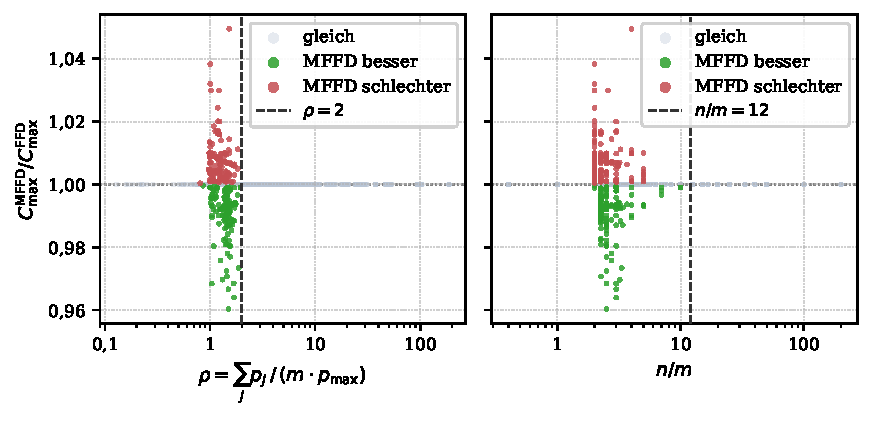
\includegraphics[width=\textwidth]{figures/abb_kollaps.pdf}
\caption{Makespan von MULTIFIT+MFFD im Verhältnis zu dem von MULTIFIT+FFD, über alle
  \EvalInstanzen{} Instanzen des Benchmarks und aufgetragen gegen
  $\rho = \sum_j p_j / (m \cdot p_{\max})$ (links) und gegen $n/m$ (rechts).
  Rechts der Linie $\rho = 2$ liegt keine Abweichung.}
\label{fig:kollaps}
\end{figure}

Tabelle~\ref{tab:kollaps} zeigt den Übergang.
Der Anteil abweichender Instanzen erreicht sein Maximum mit \EvalKollapsMaxAnteil{} im Bereich
\EvalKollapsMaxBereich{} und fällt unmittelbar unterhalb der Schwelle auf
\EvalKollapsLetzterAnteil, oberhalb von $\rho = 2$ auf null.
Die Schranke aus Lemma~\ref{lem:kollaps} ist auf diesen Datensätzen also nicht nur korrekt,
sondern wird auch fast erreicht.
Auf den \EvalRhoUnterZwei{} Instanzen mit $\rho < 2$ ist ein Unterschied möglich; wie er
ausfällt, behandelt der nächste Abschnitt.

\begin{table}[htbp]
\centering
\begin{tabular}{l r r r}
\toprule
Bereich & Instanzen & Abweichungen & Anteil \\
\midrule
$\rho < 0{,}5$ & 11 & 0 & 0{,}0\,\% \\
$0{,}5 \le \rho < 1{,}0$ & 242 & 11 & 4{,}5\,\% \\
$1{,}0 \le \rho < 1{,}25$ & 1\,790 & 140 & 7{,}8\,\% \\
$1{,}25 \le \rho < 1{,}5$ & 1\,394 & 153 & 11{,}0\,\% \\
$1{,}5 \le \rho < 1{,}75$ & 1\,253 & 68 & 5{,}4\,\% \\
$1{,}75 \le \rho < 2{,}0$ & 913 & 8 & 0{,}9\,\% \\
\midrule
$\rho \ge 2{,}0$ & \textbf{3\,489} & \textbf{0} & \textbf{0{,}0\,\%} \\
\bottomrule
\end{tabular}

\caption{Anteil der Instanzen, auf denen MULTIFIT+MFFD und MULTIFIT+FFD verschiedene Makespans
  liefern, gestaffelt nach $\rho$. Oberhalb von $\rho = 2$ tritt keine Abweichung auf
  (Lemma~\ref{lem:kollaps}).}
\label{tab:kollaps}
\end{table}

\subsection{Makespan-Vergleich}
\label{sec:makespan-vergleich}

Über alle \EvalInstanzen{} Instanzen liefert MULTIFIT+MFFD in \EvalWins{} Fällen
(\EvalWinsProzent) einen kleineren, in \EvalLosses{} Fällen (\EvalLossesProzent) einen größeren
und in \EvalTies{} Fällen (\EvalTiesProzent) denselben Makespan wie MULTIFIT+FFD
(Tabelle~\ref{tab:win-tie-loss}).
Sämtliche \EvalAbweichungen{} Abweichungen liegen bei $\rho < 2$, wie es
Lemma~\ref{lem:kollaps} verlangt.

\begin{table}[htbp]
\centering
\small
\begin{tabular}{l r r r r r r r}
\toprule
Datensatz & $N$ & MFFD besser & gleich & MFFD schlechter & \multicolumn{3}{c}{$C^{\mathrm{MFFD}}_{\max}/C^{\mathrm{FFD}}_{\max}$} \\
\cmidrule(lr){6-8}
 & & & & & Min. & Median & Max. \\
\midrule
França & 150 & 0 & 150 & 0 & 1{,}0000 & 1{,}0000 & 1{,}0000 \\
Frangioni & 780 & 1 & 775 & 4 & 0{,}9996 & 1{,}0000 & 1{,}0135 \\
Lawrinenko & 3\,499 & 146 & 3\,245 & 108 & 0{,}9603 & 1{,}0000 & 1{,}0244 \\
Berndt & 3\,059 & 17 & 3\,030 & 12 & 0{,}9667 & 1{,}0000 & 1{,}0112 \\
Planted & 1\,604 & 36 & 1\,512 & 56 & 0{,}9640 & 1{,}0000 & 1{,}0495 \\
\midrule
\textbf{Alle} & 9\,092 & 200 & 8\,712 & 180 & 0{,}9603 & 1{,}0000 & 1{,}0495 \\
\bottomrule
\end{tabular}

\caption{Vergleich der Makespans von MULTIFIT+MFFD und MULTIFIT+FFD je Datensatz. Die Zeile
  \emph{Alle} berechnet Anzahlen und Kennzahlen über alle Instanzen gemeinsam.}
\label{tab:win-tie-loss}
\end{table}

Die Abweichungen fallen in beide Richtungen aus und bleiben klein:
Das Verhältnis $C^{\mathrm{MFFD}}_{\max}/C^{\mathrm{FFD}}_{\max}$ liegt zwischen \EvalMinRatioMffdFfd{} und
\EvalMaxRatioMffdFfd{} (Abbildung~\ref{fig:ratio-verteilung}).
Auf welcher Seite sie überwiegen, hängt vom Datensatz ab: Auf Lawrinenko und Berndt liefert
MFFD häufiger den kleineren, auf Frangioni und Planted häufiger den größeren Makespan
(Tabelle~\ref{tab:win-tie-loss}).
Einen systematisch kleineren Makespan liefert MULTIFIT+MFFD auf diesen Instanzen also nicht.
Aus den Schranken~\eqref{eq:ffd-guete} und~\eqref{eq:mffd-guete} ließ sich das auch nicht
erwarten: Beide beschränken nur die Binzahl nach oben und sagen nichts über den Makespan von
MULTIFIT, und für MULTIFIT+MFFD ist keine Makespan-Schranke bewiesen.

\begin{figure}[htbp]
\centering
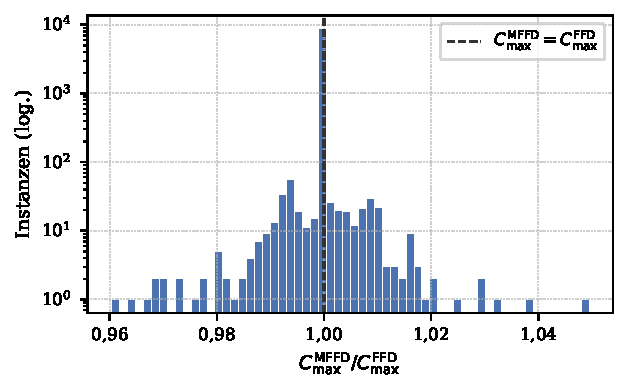
\includegraphics[width=0.72\textwidth]{figures/abb_ratio_verteilung.pdf}
\caption{Verteilung von $C^{\mathrm{MFFD}}_{\max}/C^{\mathrm{FFD}}_{\max}$ über alle \EvalInstanzen{} Instanzen
  (logarithmische $y$-Achse). Der Balken bei 1 enthält die \EvalTies{} Instanzen mit
  identischem Makespan.}
\label{fig:ratio-verteilung}
\end{figure}

\subsection{Güte gegenüber dem Optimum}
\label{sec:guete}

Auf den \EvalOptBekannt{} Instanzen mit bekanntem Optimum erreicht MULTIFIT+FFD in
\EvalOptimalFFD{} der Fälle exakt den optimalen Makespan.
Das größte beobachtete Verhältnis beträgt für beide Varianten \EvalMaxRatioOptFFD{} -
für MULTIFIT+FFD wie für MULTIFIT+MFFD -, jeweils auf einer Berndt-Instanz
(Tabelle~\ref{tab:ratio-opt}, Abbildung~\ref{fig:guete-opt}).
Beide Werte liegen unterhalb von $13/11 + 2^{-k} \approx \EvalSchrankeK$ für $k = \EvalKMax$.
Bewiesen ist diese Schranke nur für MULTIFIT+FFD, nämlich durch Theorem~\ref{thm:guete} zusammen
mit $r_m \le 13/11$ nach \textcite{cao1995}; für MULTIFIT+MFFD dient sie hier lediglich als
Vergleichslinie.

\begin{table}[htbp]
\centering
\small
\begin{tabular}{l r r r r r r r}
\toprule
Datensatz & $C^{*}_{\max}$ bekannt & \multicolumn{3}{c}{MULTIFIT+FFD} & \multicolumn{3}{c}{MULTIFIT+MFFD} \\
\cmidrule(lr){3-5}\cmidrule(lr){6-8}
 & & Mittel & Max. & $=C^{*}_{\max}$ & Mittel & Max. & $=C^{*}_{\max}$ \\
\midrule
França & 3 & 1{,}0000 & 1{,}0000 & 100{,}0\,\% & 1{,}0000 & 1{,}0000 & 100{,}0\,\% \\
Frangioni & 747 & 1{,}0066 & 1{,}0383 & 29{,}9\,\% & 1{,}0067 & 1{,}0383 & 29{,}5\,\% \\
Lawrinenko & 3\,488 & 1{,}0192 & 1{,}1080 & 27{,}5\,\% & 1{,}0190 & 1{,}1080 & 26{,}0\,\% \\
Berndt & 3\,056 & 1{,}0182 & 1{,}1221 & 19{,}1\,\% & 1{,}0181 & 1{,}1221 & 19{,}1\,\% \\
Planted & 1\,218 & 1{,}0034 & 1{,}1000 & 40{,}9\,\% & 1{,}0036 & 1{,}1000 & 40{,}1\,\% \\
\midrule
\textbf{Alle} & 8\,512 & 1{,}0154 & 1{,}1221 & 26{,}6\,\% & 1{,}0154 & 1{,}1221 & 25{,}9\,\% \\
\bottomrule
\end{tabular}

\caption{Verhältnis $C^{\mathrm{MF}}_{\max}/C^{*}_{\max}$ über die \EvalOptBekannt{} Instanzen mit
  bekanntem Optimum. \emph{Mittel} ist das arithmetische Mittel über die Instanzen, die Spalte
  $=C^{*}_{\max}$ gibt den Anteil der Instanzen an, auf denen MULTIFIT den optimalen Makespan
  erreicht. Die Zeile \emph{Alle} berechnet dieselben Kennzahlen über alle Instanzen
  gemeinsam.}
\label{tab:ratio-opt}
\end{table}

\begin{figure}[htbp]
\centering
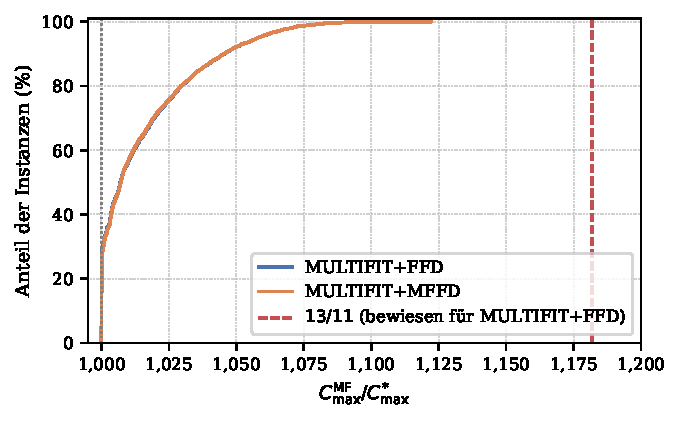
\includegraphics[width=0.78\textwidth]{figures/abb_guete_opt.pdf}
\caption{Empirische Verteilungsfunktion von $C^{\mathrm{MF}}_{\max}/C^{*}_{\max}$ über die
  \EvalOptBekannt{} Instanzen mit bekanntem Optimum. Die gestrichelte Linie markiert $13/11$;
  als Schranke bewiesen ist dieser Wert nur für MULTIFIT+FFD.}
\label{fig:guete-opt}
\end{figure}

Für die \EvalOhneOpt{} Instanzen ohne bekanntes Optimum lässt sich dieselbe Aussage über die
untere Schranke aus \eqref{eq:lb} führen: Aus $\mathrm{LB} \le C^{*}_{\max}$ folgt
$C^{\mathrm{MF}}_{\max}/C^{*}_{\max} \le C^{\mathrm{MF}}_{\max}/\mathrm{LB}$.
Auf allen \EvalLbBelegt{} dieser Instanzen gilt $C^{\mathrm{MF}}_{\max}/\mathrm{LB} \le \EvalMaxRatioLb$
und damit erst recht $C^{\mathrm{MF}}_{\max}/C^{*}_{\max} \le 13/11$
(Tabelle~\ref{tab:abdeckung}).

\begin{table}[htbp]
\centering
\begin{tabular}{l r r r r}
\toprule
Datensatz & $N$ & $C^{*}_{\max}$ bekannt & über $\mathrm{LB}$ belegt & unbestimmt \\
\midrule
França & 150 & 3 & 147 & 0 \\
Frangioni & 780 & 747 & 33 & 0 \\
Lawrinenko & 3\,499 & 3\,488 & 11 & 0 \\
Berndt & 3\,059 & 3\,056 & 3 & 0 \\
Planted & 1\,604 & 1\,218 & 386 & 0 \\
\midrule
\textbf{Gesamt} & 9\,092 & 8\,512 & 580 & 0 \\
\bottomrule
\end{tabular}

\caption{Abdeckung der gemessenen Aussage $C^{\mathrm{MF}}_{\max}/C^{*}_{\max} \le 13/11$ für
  MULTIFIT+FFD und MULTIFIT+MFFD. Für Instanzen ohne bekanntes Optimum wird sie über die untere
  Schranke~\eqref{eq:lb} belegt.}
\label{tab:abdeckung}
\end{table}

Damit gilt für jede der \EvalInstanzen{} Instanzen, dass weder MULTIFIT+FFD noch
MULTIFIT+MFFD das Verhältnis $13/11$ überschreitet; der größte über alle Instanzen mit bekanntem Optimum
gemessene Wert ist \EvalMaxRatioOpt.
Das ist eine Aussage über diese Instanzmenge: Für MULTIFIT+FFD ist sie mit der bewiesenen
Schranke verträglich, für MULTIFIT+MFFD begründet sie keine.
Die Worst-Case-Instanz von \textcite{friesen1984}, auf der MULTIFIT+FFD das Verhältnis $13/11$
exakt annimmt, ist in keinem der fünf Datensätze enthalten; Abschnitt~\ref{sec:friesen} wertet
sie deshalb gesondert für beide Subroutinen aus.

\subsection{Laufzeit}
\label{sec:laufzeit}

MFFDs zusätzliche Klassifikation kostet Laufzeit.
Der Median des instanzweisen Verhältnisses $t_{\mathrm{MFFD}}/t_{\mathrm{FFD}}$
liegt je nach Datensatz zwischen \EvalZeitMedianMin{} und
\EvalZeitMedianMax{} (Tabelle~\ref{tab:laufzeit}, Abbildung~\ref{fig:laufzeit} links).
Der Mehraufwand ist damit messbar, bleibt aber ein konstanter Faktor.

\begin{table}[htbp]
\centering
\begin{tabular}{l r r r r}
\toprule
Datensatz & Median FFD & Median MFFD & \multicolumn{2}{c}{$t_{\mathrm{MFFD}}/t_{\mathrm{FFD}}$} \\
\cmidrule(lr){4-5}
 & (ms) & (ms) & Median & 95.\ Perzentil \\
\midrule
França & 1{,}600 & 1{,}982 & 1{,}201 & 1{,}837 \\
Frangioni & 1{,}630 & 2{,}000 & 1{,}173 & 1{,}646 \\
Lawrinenko & 2{,}010 & 1{,}952 & 1{,}037 & 1{,}374 \\
Berndt & 0{,}339 & 0{,}498 & 1{,}522 & 2{,}078 \\
Planted & 1{,}743 & 2{,}027 & 1{,}154 & 1{,}855 \\
\midrule
\textbf{Alle} & 1{,}051 & 1{,}095 & 1{,}217 & 1{,}965 \\
\bottomrule
\end{tabular}

\caption{Laufzeit eines vollständigen MULTIFIT-Laufs ($k = 10$) und paarweises Verhältnis
  beider Subroutinen je Instanz. Die Zeile \emph{Alle} gibt Median und Perzentil über
  alle Instanzen gemeinsam an, nicht einen Mittelwert der Datensatzzeilen.}
\label{tab:laufzeit}
\end{table}

\begin{figure}[htbp]
\centering
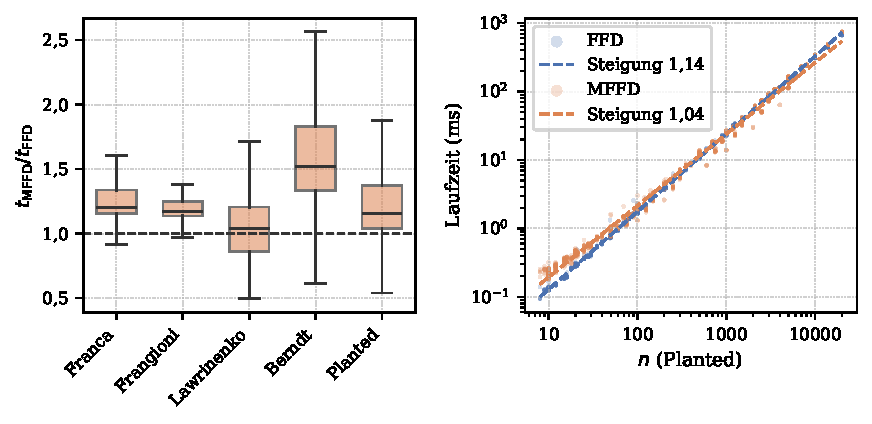
\includegraphics[width=\textwidth]{figures/abb_laufzeit.pdf}
\caption{Links: paarweises Laufzeitverhältnis je Datensatz (ohne Ausreißer).
  Rechts: Laufzeit gegen $n$ auf dem Planted-Datensatz, dessen $n$ sich über drei
  Größenordnungen erstreckt, mit Ausgleichsgeraden im doppelt-logarithmischen Maßstab.}
\label{fig:laufzeit}
\end{figure}

Das Wachstum in $n$ unterscheidet sich zwischen beiden Subroutinen nicht wesentlich:
Auf dem Planted-Datensatz, dem einzigen mit einem $n$-Bereich über drei Größenordnungen,
beträgt die Steigung der Ausgleichsgeraden im doppelt-logarithmischen Maßstab
\EvalSteigungFFD{} für FFD und \EvalSteigungMFFD{} für MFFD
(Abbildung~\ref{fig:laufzeit} rechts).
Eine Steigung nahe 1 ist mit der Laufzeit $O(n \log n)$ beider Implementierungen verträglich.
Zur Einordnung der absoluten Werte siehe Abschnitt~\ref{sec:grenzen}.

\subsection{Sensitivität gegenüber der Binärsuchtiefe}
\label{sec:k-sensitivitaet}

Nach Theorem~\ref{thm:guete} gilt für MULTIFIT+FFD $R_m(\mathrm{MF}(k)) \le r_m + 2^{-k}$: Der
additive Term, welcher auf die Binärsuche entfällt, halbiert sich mit jedem Halbierungsschritt.
Um zu messen, ab welchem $k$ sich das Ergebnis auf den Benchmark-Instanzen nicht mehr ändert,
wurde MULTIFIT für $k = 1, \ldots, 10$ über alle \EvalInstanzen{} Instanzen ausgeführt.

Das gemessene Maximum liegt für beide Subroutinen bei jeder Tiefe unterhalb von
$13/11 + 2^{-k}$, der für MULTIFIT+FFD bewiesenen Schranke
(Tabelle~\ref{tab:k-sensitivitaet}, Abbildung~\ref{fig:k-sensitivitaet} rechts):
bei $k = 1$ sind es \EvalKMaxEins{} gegenüber \EvalKSchrankeEins{}, bei
$k = \EvalKStabilMax$ dann \EvalKMaxZehn{} gegenüber \EvalKSchrankeStabil{} und bei
$k = \EvalKMax$ \EvalKMaxZehn{} gegenüber \EvalSchrankeK.

\begin{figure}[htbp]
\centering
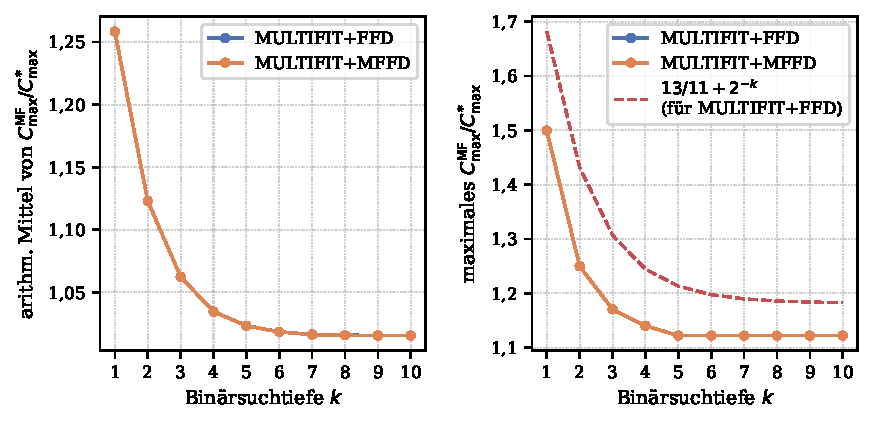
\includegraphics[width=\textwidth]{figures/abb_k_sensitivitaet.pdf}
\caption{Arithmetisches Mittel (links) und Maximum (rechts) des Verhältnisses
  $C^{\mathrm{MF}}_{\max}/C^{*}_{\max}$ in Abhängigkeit der Binärsuchtiefe $k$ über die
  \EvalOptBekannt{} Instanzen mit bekanntem Optimum. Rechts zusätzlich die für MULTIFIT+FFD
  bewiesene Schranke $13/11 + 2^{-k}$ nach \textcite{cao1995}.}
\label{fig:k-sensitivitaet}
\end{figure}
Ab $k = \EvalKStabilMax$ ändert sich das Maximum nicht mehr; der Mittelwert sinkt dagegen
bis $k = \EvalKMax$ weiter, von \EvalKMittelEins{} bei $k = 1$ auf \EvalKMittelZehn.

\begin{table}[htbp]
\centering
\small
\begin{tabular}{r r r r r r r}
\toprule
$k$ & \multicolumn{2}{c}{MULTIFIT+FFD} & \multicolumn{2}{c}{MULTIFIT+MFFD} & $13/11 + 2^{-k}$ & stabil \\
\cmidrule(lr){2-3}\cmidrule(lr){4-5}
 & Mittel & Max. & Mittel & Max. & & \\
\midrule
1 & 1{,}2584 & 1{,}4997 & 1{,}2584 & 1{,}4997 & 1{,}6818 & 0{,}2\,\% \\
2 & 1{,}1230 & 1{,}2497 & 1{,}1230 & 1{,}2497 & 1{,}4318 & 1{,}9\,\% \\
3 & 1{,}0624 & 1{,}1705 & 1{,}0624 & 1{,}1705 & 1{,}3068 & 6{,}3\,\% \\
4 & 1{,}0346 & 1{,}1400 & 1{,}0345 & 1{,}1400 & 1{,}2443 & 14{,}6\,\% \\
5 & 1{,}0233 & 1{,}1221 & 1{,}0232 & 1{,}1221 & 1{,}2131 & 27{,}7\,\% \\
6 & 1{,}0184 & 1{,}1221 & 1{,}0183 & 1{,}1221 & 1{,}1974 & 48{,}0\,\% \\
7 & 1{,}0163 & 1{,}1221 & 1{,}0162 & 1{,}1221 & 1{,}1896 & 69{,}6\,\% \\
8 & 1{,}0157 & 1{,}1221 & 1{,}0156 & 1{,}1221 & 1{,}1857 & 83{,}1\,\% \\
9 & 1{,}0155 & 1{,}1221 & 1{,}0155 & 1{,}1221 & 1{,}1838 & 91{,}5\,\% \\
10 & 1{,}0154 & 1{,}1221 & 1{,}0154 & 1{,}1221 & 1{,}1828 & 100{,}0\,\% \\
\bottomrule
\end{tabular}

\caption{Verhältnis $C^{\mathrm{MF}}_{\max}/C^{*}_{\max}$ in Abhängigkeit der Binärsuchtiefe $k$
  über die \EvalOptBekannt{} Instanzen mit bekanntem Optimum. \emph{Mittel} ist das
  arithmetische Mittel, $13/11 + 2^{-k}$ die für MULTIFIT+FFD bewiesene Schranke.
  Die letzte Spalte gibt den Anteil der Instanzen an, auf denen MULTIFIT+FFD bei $k$ bereits
  denselben Makespan liefert wie bei $k = \EvalKMax$ (die letzte Zeile daher definitionsgemäß
  $100\,\%$).}
\label{tab:k-sensitivitaet}
\end{table}

Auch bei $k = \EvalKMax$ hat sich der Makespan nicht auf allen Instanzen stabilisiert: Bei
MULTIFIT+FFD stimmt er auf \EvalKStabilNeun{} der Instanzen bei $k = 9$ mit dem bei
$k = \EvalKMax$ überein, auf den übrigen ändert er sich im letzten Halbierungsschritt noch.
Da die Suche reellwertige Kapazitäten testet, schrumpft das Suchintervall mit jedem Schritt,
wird aber nie leer; ein größeres $k$ kann folglich eine noch kleinere akzeptierte Kapazität und
damit einen kleineren Makespan liefern.
Die ganzzahlige Suche aus Abschnitt~\ref{sec:hm} endet dagegen, sobald sich untere und obere
Grenze des Intervalls treffen.

Der Makespan fällt allerdings nicht durchgängig monoton in $k$.
MULTIFIT verkleinert die Kapazitätsschranke $C$, nicht den tatsächlich erreichten Makespan:
Passt eine Packung mit kleinerem $C$ noch in $m$ Bins, wird sie übernommen, auch wenn ihre
größte Binlast über der der bisher gespeicherten Packung liegt.
Über alle \EvalInstanzen{} Instanzen und alle Übergänge $k \to k+1$ zählt die Messung
\EvalKNichtMonotonFFD{} solche Fälle bei MULTIFIT+FFD und \EvalKNichtMonotonMFFD{} bei
MULTIFIT+MFFD; die größte dabei gemessene Verschlechterung beträgt \EvalKNichtMonotonMax{}
(Instanz \texttt{\EvalKNichtMonotonInstanz}: Makespan \EvalKNichtMonotonVorher{} bei
$k = \EvalKNichtMonotonKVorher$, \EvalKNichtMonotonNachher{} bei
$k = \EvalKNichtMonotonKNachher$, gemessen mit \EvalKNichtMonotonAlg).


\subsection{Fallstudie: die Friesen-Instanz}
\label{sec:friesen}

Keine Instanz der fünf Datensätze erreicht das Verhältnis $13/11$.
Die von \textcite{friesen1984} angegebene Instanz, auf der MULTIFIT+FFD diesen Wert
annimmt, erlaubt es, das Verhalten beider Subroutinen an einem Extremfall nachzuvollziehen.

Die Instanz besteht aus $n = 39$ Aufgaben auf $m = 13$ Maschinen:
achtmal $(40, 13, 13)$, dreimal $(25, 25, 16)$ und zweimal $(25, 24, 17)$.
Die Gesamtlast ist $858 = 13 \cdot 66$, und es existiert eine Zuordnung, bei der jede Maschine
exakt 66 Lasteinheiten erhält; also $C^{*}_{\max} = 66$.
Wegen $\rho = 858 / (13 \cdot 40) = 1{,}65 < 2$ dürfen sich die Subroutinen nach
Lemma~\ref{lem:kollaps} unterscheiden - und sie tun es:

\begin{center}
\begin{tabular}{l r r}
\toprule
 & MULTIFIT+FFD & MULTIFIT+MFFD \\
\midrule
Makespan ($k = 10$)        & 78     & 75 \\
Verhältnis zu $C^{*}_{\max}$ & $78/66 = 13/11$ & $75/66 \approx 1{,}1364$ \\
\bottomrule
\end{tabular}
\end{center}

Der Unterschied entsteht bei der Kapazität $C = 75$.
Dort ist $C/2 = 37{,}5$, sodass die acht 40er-Aufgaben \emph{large} sind, und $C/6 = 12{,}5$,
sodass auch die 13er-Aufgaben noch \emph{small} sind.
Phase~3 von MFFD kombiniert daher jeden 40er-Bin mit einer 13er-Aufgabe und einer weiteren
passenden Aufgabe; MFFD packt die Instanz in 13~Bins, FFD benötigt 14.
Bei $C = 78$ dagegen ist $C/6 = 13$ und die 13er-Aufgaben sind \emph{tiny};
Phase~3 bleibt für sie wirkungslos.

Abbildung~\ref{fig:friesen-binzahl} zeigt die Binzahlen beider Subroutinen für jede ganzzahlige
Kapazität von $C^{*}_{\max} = 66$ bis $90$.
FFD benötigt für jede Kapazität von 66 bis 77 vierzehn Bins und fällt bei $C = 78$ auf elf;
die Binärsuche akzeptiert daher erst $C = 78$.
MFFD kommt bereits ab $C = 75$ mit 13~Bins aus, weshalb MULTIFIT+MFFD gegen 75 konvergiert.
Erreicht wird dieser Wert ab $k \ge 6$; bei kleinerem $k$ liegt das Suchintervall noch zu grob
(bei $k = 5$ ergibt sich 76).

\begin{figure}[htbp]
\centering
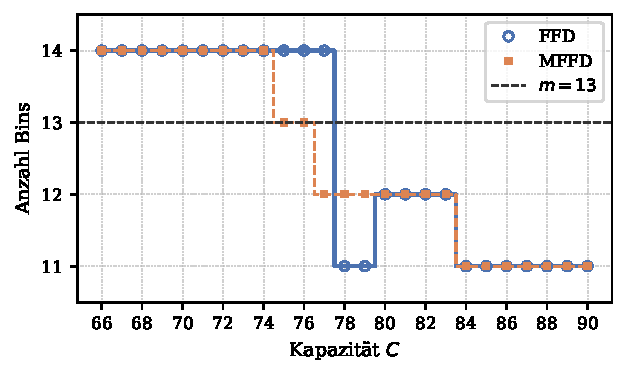
\includegraphics[width=0.72\textwidth]{figures/abb_friesen_binzahl.pdf}
\caption{Anzahl der Bins von FFD und MFFD auf der Friesen-Instanz für jede ganzzahlige Kapazität
  $C = 66, \ldots, 90$. MULTIFIT akzeptiert eine Kapazität, wenn die Binzahl auf oder unter der
  gestrichelten Linie $m = 13$ liegt. Beim Übergang von $C = 79$ auf $C = 80$ steigt die Binzahl
  von FFD.}
\label{fig:friesen-binzahl}
\end{figure}

Der Übergang von $C = 79$ auf $C = 80$ belegt zugleich, dass die Binzahl von FFD nicht monoton
in $C$ fällt.
Bei $C = 79$ kombiniert First Fit jede 40er-Aufgabe mit einer 25er- und einer 13er-Aufgabe zur
Last 78 und füllt so elf Bins.
Bei $C = 80$ passen zwei 40er-Aufgaben gemeinsam in einen Bin; dadurch entfällt diese
Kombination, die 25er-Aufgaben belegen eigene Bins, und am Ende bleibt eine 13er-Aufgabe
allein in einem zwölften Bin.
Erst ab $C = 84$ kommt FFD wieder mit elf Bins aus.
Auf dieser Instanz bleibt das ohne Folgen für MULTIFIT, da beide Werte unter $m = 13$ liegen und
das Akzeptanzkriterium $\mathrm{FFD}[\Gamma, C] \le m$ damit in beiden Fällen erfüllt ist.

Dass MULTIFIT+MFFD auf dieser Instanz besser abschneidet, sagt nichts über sein
Worst-Case-Verhältnis aus.
Ob $r_m(\mathrm{MF{+}MFFD}) < 13/11$ gilt, ist offen.

\subsection{Grenzen der Auswertung}
\label{sec:grenzen}

\begin{itemize}
  \item \textbf{Herkunft der Optima.} Die OPT-Werte für Frangioni, Lawrinenko, Berndt und einen
    Teil der Planted-Instanzen stammen aus \textcite{akram2025} und wurden nicht selbst
    nachgerechnet. Sie gehen in Abschnitt~\ref{sec:guete} unmittelbar in das Verhältnis
    $C^{\mathrm{MF}}_{\max}/C^{*}_{\max}$ ein. Die über \eqref{eq:lb} geführte Argumentation ist davon
    unabhängig.
  \item \textbf{Laufzeitmessung.} Jede Instanz wurde einmal gemessen. Die Werte in
    Tabelle~\ref{tab:laufzeit} sind Mediane über viele Instanzen, aber keine Mittel über
    wiederholte Läufe derselben Instanz; einzelne Werte enthalten Messrauschen.
    Die absoluten Zeiten gelten für die beschriebene Python-Implementierung und Umgebung.
  \item \textbf{Abdeckung des Parameterraums.} \EvalRhoZweiProzent{} der Instanzen erfüllen
    $\rho \ge 2$ und sind nach Lemma~\ref{lem:kollaps} für den Subroutinenvergleich ohne
    Aussagekraft. Die verbleibenden \EvalRhoUnterZwei{} Instanzen konzentrieren sich auf
    $\rho \in [1;\,2]$; sehr kleine Werte $\rho < 0{,}5$ kommen nur elfmal vor.
  \item \textbf{Reichweite der Ergebnisse.} Alle Angaben beziehen sich auf $k = 10$ und auf
    diese fünf Datensätze. Aus dem Ausbleiben eines Verhältnisses über $13/11$ folgt keine
    schärfere Schranke, und aus den beobachteten Abweichungen folgt keine Aussage über das
    Worst-Case-Verhalten von MULTIFIT+MFFD.
\end{itemize}

\section{High-Multiplicity-Subroutinen}
\label{sec:hm}

Kommen in einer Instanz nur $d$ verschiedene Aufgabengrößen vor, lässt sie sich kompakter
kodieren: Statt der $n$ einzelnen Größen genügen die verschiedenen Größen $p_1, \ldots, p_d$ und
ihre Vielfachheiten $u_1, \ldots, u_d$ (High-Multiplicity-Darstellung,
Abschnitt~\ref{sec:jansen}).
Die Kodierungslänge liegt dann in $O\bigl(d \cdot (\log p_{\max} + \log n)\bigr)$, während die
Liste der Aufgabengrößen $n$ Zahlen umfasst.
Erst in dieser Kodierung ist eine Laufzeit polynomiell in $\log n$, wie sie
Abschnitt~\ref{sub:jansen-laufzeit} angibt, überhaupt möglich, denn schon das Einlesen von $n$
einzelnen Größen kostet $\Omega(n)$.
Kapitel~\ref{kap:alternative} stellt neben MFFD drei Subroutinen vor, welche diese Darstellung
ausnutzen: den $\mathrm{OPT}+1$-Algorithmus von \textcite{jansen_solisoba2010}
(Abschnitt~\ref{sec:jansen}), seine $\varepsilon$-duale Modifikation
(Abschnitt~\ref{sub:eps_dual}) und das Konfigurations-LP von Gilmore und Gomory
(Abschnitt~\ref{sec:gg-lp}).
Dieser Abschnitt misst, was sie als Subroutine in MULTIFIT leisten.

Gegenüber Abschnitt~\ref{sec:greedy} kommt dabei ein Hilfsmittel hinzu: Dasselbe
Konfigurationsprogramm liefert in ganzzahliger Fassung $\mathrm{OPT}[\Gamma, C]$ exakt.
Bei jeder getesteten Kapazität ist damit bekannt, wie viele Bins mindestens nötig sind -
die Schranken aus Kapitel~\ref{kap:alternative} lassen sich nachrechnen, statt sie nur zu
zitieren.

\subsection{Datensätze}
\label{sub:hm-datensaetze}

Die fünf Datensätze aus Abschnitt~\ref{sec:benchmarks} sind für diesen Vergleich ungeeignet:
Ihre Instanzen enthalten im Median zwischen \HmDBenchMedianMin{} und \HmDBenchMedianMax{}
verschiedene Aufgabengrößen, im Maximum \HmDBenchMax.
Nach Abschnitt~\ref{sub:anwendbarkeit} setzen die Verfahren ein konstantes und sehr kleines $d$
voraus.
Für den Vergleich wurden deshalb zwei Datensätze erzeugt.

\paragraph{HM-Gitter.}
Der erste Datensatz - HM steht für High Multiplicity - umfasst
\HmInstanzen{} Instanzen aus einem vollständig balancierten Gitter:
$d \in \{\HmDMin,\dots,\HmDMax\}$ verschiedene Aufgabengrößen, drei Szenarien für deren
Verteilung, drei Maschinenzahlen zwischen \HmMMin{} und \HmMMax{} und drei Verhältnisse $n/m$
mit je zehn Instanzen (Tabelle~\ref{tab:hm-datensatz}).
Die Größenbereiche sind aus $\varepsilon = 1/(2d-1)$ abgeleitet, also aus der
Groß-Klein-Schwelle des $\mathrm{OPT}+1$-Algorithmus selbst.
Die Instanzen sind klein ($n$ zwischen \HmNMin{} und \HmNMax); variiert werden $d$, $m$ und
$n/m$, nicht die Vielfachheiten.

\begin{table}[htbp]
\centering
\begin{tabular}{lrrrrr}
\toprule
Szenario & Instanzen & $n$ & $m$ & $d$ & $\rho$ \\
\midrule
Dense & 360 & 15--160 & 5--20 & 3--6 & 1{,}34--7{,}74 \\
Mixed & 360 & 15--160 & 5--20 & 3--6 & 0{,}52--7{,}74 \\
Asymmetric & 360 & 15--160 & 5--20 & 3--6 & 0{,}67--7{,}00 \\
\midrule
Gesamt & 1\,080 & 15--160 & 5--20 & 3--6 & 0{,}52--7{,}74 \\
\bottomrule
\end{tabular}

\caption{Aufbau des HM-Gitters. Je Szenario \HmInstanzenSzenario{} Instanzen aus
  $d \in \{\HmDMin,\dots,\HmDMax\}$, drei Maschinenzahlen, drei Verhältnissen $n/m$ und zehn
  Instanzen je Kombination.}
\label{tab:hm-datensatz}
\end{table}

\paragraph{HM-Skalierung.}
\HmSkalInstanzen{} Instanzen, die die fehlende Achse ergänzen: $d \in \{3,4\}$, dieselben drei
Szenarien, $n$ von \HmSkalNMin{} bis \HmSkalNMax{} bei festem $n/m = \HmSkalRatio$ (also $m$ bis
\HmSkalMMax), je fünf Instanzen.
Das feste Verhältnis ist konstruktionsbedingt nötig: Bei festem $m$ wüchse mit $n$ auch das
Startintervall der Binärsuche~\eqref{eq:startintervall} und mit ihm die Zahl der
Konfigurationen; bei festem $n/m$ bleibt die getestete Kapazität in derselben Größenordnung, und
es wachsen allein die Vielfachheiten.
Damit ein Konfigurations-LP je Kapazität lösbar bleibt, verwirft der Generator jede
Größenkombination, bei welcher die obere Schranke $\prod_{i=1}^{d} (\lfloor C/p_i \rfloor + 1)$ für die
Zahl der Konfigurationen über \HmSkalBudget{} liegt.
Dabei ist $C = \HmSkalRatio\,\bar{p} + p_{\max}$ mit dem Mittelwert $\bar{p}$ der $d$ Größen,
eine von $n$ unabhängige Näherung der oberen Grenze des Startintervalls.
Diese Grenze beschränkt $d$: Schon für $d = \HmSkalDLuecke$ hält im Szenario
\HmSkalSzenarioLuecke{} keine von \HmSkalZuege{} zufällig gezogenen Größenkombinationen sie ein,
während für $d \le \HmSkalDMaxAlle$ in allen drei Szenarien zulässige Kombinationen existieren.
Dieser Datensatz wird nur in Abschnitt~\ref{sub:hm-skalierung} ausgewertet.

\paragraph{Referenzwerte.}
Für alle \HmInstanzen{} Instanzen des HM-Gitters wurde $C^{*}_{\max}(\Gamma)$ für diese Arbeit
exakt bestimmt.
Nach Lemma~\ref{lem:dualitaet} ist
$C^{*}_{\max}(\Gamma) = \min\{C : \mathrm{OPT}[\Gamma, C] \le m\}$, und da
$\mathrm{OPT}[\Gamma,\cdot\,]$ monoton fällt, findet eine Binärsuche über $C$ diesen Wert,
sobald sich $\mathrm{OPT}[\Gamma, C]$ berechnen lässt.
Das leistet das ganzzahlige Konfigurationsprogramm; seine Größe hängt nur von $d$ und $C$ ab,
nicht von $n$ oder $m$.
Alle \HmInstanzen{} Werte sind auf diesem Weg als optimal nachgewiesen.

\paragraph{Degenerierte Instanzen.}
\HmDegeneriert{} Instanzen des HM-Gitters erfüllen $\rho(\Gamma) < 1$, bei ihnen übersteigt die
größte Aufgabe also die mittlere Maschinenlast; bei \HmDegOptPMax{} von ihnen ist
$C^{*}_{\max}(\Gamma) = p_{\max}$, die untere Schranke aus Lemma~\ref{lem:untere-schranken} wird
dort angenommen.
Auf diesen Instanzen erreichen \HmDegAlleOptimal{} fünf Subroutinen den optimalen Makespan; sie
trennen die Verfahren nicht und bleiben in den Gütevergleichen unberücksichtigt.

\subsection{Versuchsaufbau}
\label{sub:hm-aufbau}

\paragraph{Subroutinen.}
Gemessen werden fünf Subroutinen: FFD als Grundlinie, der $\mathrm{OPT}+1$-Algorithmus ($\mathrm{J}$), seine
$\varepsilon$-duale Variante ($\mathrm{J}_\varepsilon$), das Konfigurations-LP mit Rundung
($\mathrm{GG}$) und dasselbe Programm in ganzzahliger Fassung ($\mathrm{GG}$-IP).
Letzteres löst $\mathrm{OPT}[\Gamma, C]$ exakt und dient als Referenzlinie.

\paragraph{Implementierungsvarianten der beiden Jansen-Algorithmen.}
$\mathrm{J}$ und $\mathrm{J}_\varepsilon$ unterscheiden sich nicht nur im Rundungsschritt,
sondern auch in der Anzahl der Aufrufe des Lösers.
Für die Laufzeitmessung in Abschnitt~\ref{sub:hm-laufzeit} ist das der entscheidende
Unterschied.
$\mathrm{J}$ wird in der publizierten Form gemessen.
Schritt~2 bestimmt dort das kleinste $m^*$, für welches das MILP zulässig ist, per Binärsuche über
$\{1, \ldots, n\}$ (Abschnitt~\ref{sub:jansen-implementierung}); jeder Suchschritt löst ein MILP
und halbiert das Intervall, sodass je Kapazität $O(\log n)$ MILP-Aufrufe anfallen.
Nötig ist diese Suche, obwohl MULTIFIT die Maschinenzahl $m$ vorgibt: Ein einzelner Aufruf mit
$m$ an Stelle von $m^*$ kann wegen des zusätzlichen Bins aus Schritt~3 insgesamt $m+1$ Bins
ausgeben und die Kapazität verwerfen, obwohl die publizierte Form mit $m^* < m$ höchstens $m$
Bins ausgibt und sie annimmt (Abschnitt~\ref{sub:eps_dual}).
$\mathrm{J}_\varepsilon$ verteilt die Reste dagegen auf die bereits geöffneten Bins und wird
deshalb in der Fassung aus Abschnitt~\ref{sub:eps_dual} ohne innere Binärsuche gemessen: Je
Kapazität wird das MILP einmal mit der Nebenbedingung $\sum_b y_b \le m$ gelöst.

\paragraph{Parameter.}
Alle fünf Subroutinen laufen mit $k = 10$ wie in Abschnitt~\ref{sec:versuchsaufbau}, aber mit
\emph{ganzzahligen} Kapazitäten.
Da alle Aufgabengrößen ganzzahlig sind, ist jede Binlast ganzzahlig; eine Kapazität $C$ lässt
daher dieselben Packungen zu wie $\lfloor C \rfloor$.
Die Binärsuche testet deshalb nur ganze Zahlen, setzt nach einer Ablehnung von $C$ die untere
Grenze auf $C+1$ und endet, sobald sich untere und obere Grenze treffen.
So prüft jeder Aufruf der Subroutine eine andere Kapazität.
FFD wird deshalb in dieser Variante neu gemessen und nicht aus Abschnitt~\ref{sec:laufzeit}
übernommen.
Jede Instanz wird von allen fünf Subroutinen im selben Prozess bearbeitet.

\paragraph{Messumgebung.}
Umgebung wie in Abschnitt~\ref{sec:versuchsaufbau}; die vier übrigen Subroutinen lösen ihre
Programme mit Gurobi~13.0.2.
Die Laufzeit umfasst den vollständigen Lauf von MULTIFIT einschließlich aller Aufrufe des
Lösers, nicht einzelne Packvorgänge.

\paragraph{Reproduktion.}
Die Messung übernimmt \texttt{run\_hm\_benchmark.py} und legt zwei Dateien ab: eine Zeile je
Instanz mit Makespan und Laufzeit jeder Subroutine sowie eine Zeile je Tripel aus Instanz,
getesteter Kapazität und Subroutine mit den Kennzahlen des jeweiligen Aufrufs.
Daraus erzeugen \texttt{summary\_tables\_hm.py} die Tabellen und Kennzahlen sowie
\texttt{thesis\_figures\_hm.py} die Abbildungen.
Diese Kette ist von der aus Abschnitt~\ref{sec:versuchsaufbau} getrennt.

\subsection{Güte gegenüber dem Optimum}
\label{sub:hm-guete}

Tabelle~\ref{tab:hm-ratio-opt} und Abbildung~\ref{fig:hm-guete} zeigen den Abstand zum Optimum.
MULTIFIT+FFD erreicht auf \HmOptimalffd{} der Instanzen den optimalen Makespan, im schlechtesten
Fall das Verhältnis \HmMaxRatioOptffd.
Die drei High-Multiplicity-Subroutinen liegen darüber: \HmOptimaljansen{} für $\mathrm{J}$,
\HmOptimaljansendual{} für $\mathrm{J}_\varepsilon$ und \HmOptimalgglp{} für $\mathrm{GG}$; ihre
größten Verhältnisse liegen zwischen \HmMaxRatioOptjansendual{} und \HmMaxRatioOptjansen.

\begin{table}[htbp]
\centering
\small
\begin{tabular}{lrrrrrr}
\toprule
& & \multicolumn{5}{c}{Maximum von $C^{\mathrm{MF}}_{\max}/C^{*}_{\max}$} \\
\cmidrule(lr){3-7}
$d$ & Instanzen & FFD & Jansen OPT+1 & Jansen $\varepsilon$-dual & GG-LP & GG-IP (exakt) \\
\midrule
3 & 270 & 1{,}1429 & 1{,}0317 & 1{,}0303 & 1{,}0303 & 1{,}0000 \\
4 & 271 & 1{,}1327 & 1{,}0292 & 1{,}0216 & 1{,}0254 & 1{,}0000 \\
5 & 259 & 1{,}0920 & 1{,}0247 & 1{,}0232 & 1{,}0296 & 1{,}0000 \\
6 & 256 & 1{,}1154 & 1{,}0116 & 1{,}0217 & 1{,}0317 & 1{,}0000 \\
\midrule
alle $d$ & 1\,056 & 1{,}1429 & 1{,}0317 & 1{,}0303 & 1{,}0317 & 1{,}0000 \\
\bottomrule
\end{tabular}

\caption{Größtes Verhältnis $C^{\mathrm{MF}}_{\max}/C^{*}_{\max}$ je Subroutine, gestaffelt nach der
  Anzahl $d$ verschiedener Aufgabengrößen. Die \HmDegeneriert{} Instanzen mit $\rho < 1$ sind
  ausgenommen.}
\label{tab:hm-ratio-opt}
\end{table}

\begin{figure}[htbp]
\centering
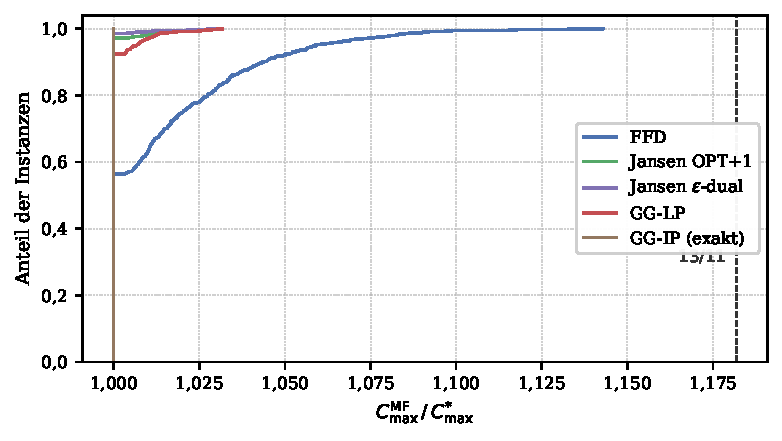
\includegraphics[width=0.90\textwidth]{figures/abb_hm_guete.pdf}
\caption{Empirische Verteilungsfunktion von $C^{\mathrm{MF}}_{\max}/C^{*}_{\max}$ je Subroutine.
  Die Verteilung von GG-IP liegt konstruktionsbedingt vollständig bei 1.}
\label{fig:hm-guete}
\end{figure}

Die Spalten der vier nicht exakten Subroutinen sind dabei unterschiedlich zu lesen.
Zwei von ihnen prüfen je eine bewiesene, instanzunabhängige Schranke nach: die Spalte zu
MULTIFIT+FFD den Wert $13/11 + 2^{-k} \approx \HmSchrankeK$ nach \textcite{cao1995}, die
Spalte zu MULTIFIT+$\mathrm{J}_\varepsilon$ den Wert $(1+\varepsilon)(1+2^{-k})$ nach
Korollar~\ref{kor:multifit-jansen-dual}, wobei $\varepsilon = 1/(2d-1)$ hier zwischen
\HmEpsTheorieMin{} und \HmEpsTheorieMax{} liegt.
Für MULTIFIT+$\mathrm{J}$ beziffert Abschnitt~\ref{sub:anwendbarkeit} die Güte durch den
Quotienten $C^{*}_{\max}(\Gamma, m-1)/C^{*}_{\max}(\Gamma, m)$, der im Allgemeinen bis
zu $2$ betragen kann - eine Schranke, die von der Instanz abhängt.
Für das Konfigurations-LP trägt dasselbe Argument mit $\mathrm{GG}[\Gamma,C] \le
\mathrm{OPT}[\Gamma,C] + d - 1$ nur die schwächere Schranke
$C^{*}_{\max}(\Gamma, m-d+1)/C^{*}_{\max}(\Gamma, m)$.
Eine instanzunabhängige Schranke liefert Abschnitt~\ref{sub:gg-multifit} dagegen nicht: Die
Schlussweise hinter der Schranke $13/11$ verlangt eine Konstante $r$, für die jede Kapazität
$C \ge r \cdot C^{*}_{\max}(\Gamma)$ mit $m$ Bins auskommt
(Implikation~\eqref{eq:ffd-akzeptiert}); Lemma~\ref{lem:gg-rundung} lässt dort $m + d - 1$ zu.
Für das Konfigurations-LP sind die gemessenen Werte damit die einzige verfügbare Aussage über
das Verhältnis auf diesen Instanzen.

Der direkte Vergleich (Tabelle~\ref{tab:hm-paare}, Abbildung~\ref{fig:hm-paare}) fällt nicht
einheitlich aus.
Gegenüber MULTIFIT+FFD liefert MULTIFIT+$\mathrm{J}$ auf \HmJansenBesserFFD{} Instanzen den
kleineren Makespan - und auf \HmJansenSchlechterFFD{} den größeren.
Die kleinere obere Schranke für die Binzahl ($\mathrm{OPT}+1$ gegenüber~\eqref{eq:ffd-guete})
garantiert also keinen kleineren Makespan; woran das auf diesen Instanzen liegt, zeigt
Abschnitt~\ref{sub:hm-garantien}.

\begin{table}[htbp]
\centering
\small
\begin{tabular}{llrrrr}
\toprule
Referenz $A$ & Kandidat $B$ & $B$ besser & gleich & $B$ schlechter & Instanzen \\
\midrule
FFD & Jansen OPT+1 & 453 & 619 & 8 & 1\,080 \\
FFD & Jansen $\varepsilon$-dual & 457 & 618 & 5 & 1\,080 \\
FFD & GG-LP & 446 & 633 & 1 & 1\,080 \\
FFD & GG-IP (exakt) & 461 & 619 & 0 & 1\,080 \\
Jansen OPT+1 & Jansen $\varepsilon$-dual & 23 & 1\,048 & 9 & 1\,080 \\
Jansen OPT+1 & GG-LP & 24 & 984 & 72 & 1\,080 \\
Jansen OPT+1 & GG-IP (exakt) & 29 & 1\,051 & 0 & 1\,080 \\
Jansen $\varepsilon$-dual & GG-LP & 13 & 989 & 78 & 1\,080 \\
Jansen $\varepsilon$-dual & GG-IP (exakt) & 15 & 1\,065 & 0 & 1\,080 \\
GG-LP & GG-IP (exakt) & 80 & 1\,000 & 0 & 1\,080 \\
\bottomrule
\end{tabular}

\caption{Paarweiser Vergleich der Makespans über alle \HmInstanzen{} Instanzen des HM-Gitters.}
\label{tab:hm-paare}
\end{table}

\begin{figure}[htbp]
\centering
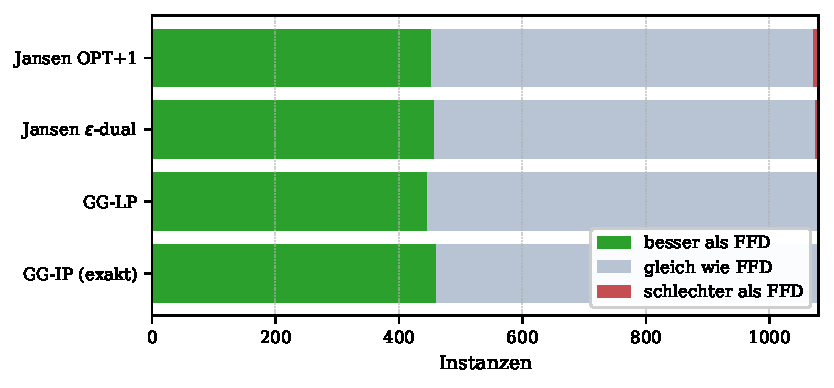
\includegraphics[width=0.96\textwidth]{figures/abb_hm_paare.pdf}
\caption{Jede Subroutine gegen die Grundlinie MULTIFIT+FFD.}
\label{fig:hm-paare}
\end{figure}

\subsection{Die Garantien im Test}
\label{sub:hm-garantien}

Weil GG-IP $\mathrm{OPT}[\Gamma, C]$ bei jeder getesteten Kapazität liefert, lassen sich
die Schranken aus Kapitel~\ref{kap:alternative} unmittelbar nachrechnen.

Für den $\mathrm{OPT}+1$-Algorithmus gilt in allen \HmJansenVergleiche{} verglichenen Aufrufen
$\mathrm{J}[\Gamma,C] - \mathrm{OPT}[\Gamma,C] \in \{0,1\}$, wie es
\textcite{jansen_solisoba2010} garantiert; der Wert 1 tritt in \HmJansenPlusEins{} Fällen auf
(\HmJansenUeberOpt), sonst ist die Packung optimal.

Für das Konfigurations-LP erlaubt Lemma~\ref{lem:gg-rundung} den additiven Term $d-1$, hier also
bis zu \HmDMinusEins.
Gemessen wird er nicht annähernd erreicht: Über \HmGGVergleiche{} Aufrufe ist
$\mathrm{GG}[\Gamma,C] - \mathrm{OPT}[\Gamma,C]$ höchstens \HmGGMaxUeberOpt{} und in
\HmGGPlusEins{} Fällen überhaupt von null verschieden.
Auch der Abstand zur LP-Schranke bleibt klein: In \HmGGOhneVerlust{} der Aufrufe gilt
$\mathrm{GG}[\Gamma,C] = \lceil \mathrm{LP}[\Gamma,C] \rceil$, der größte beobachtete Abstand ist
\HmGGRundungsverlustMax.

Nicht ursächlich dafür ist die Trägerschranke $|F| \le d$ aus Lemma~\ref{lem:gg-ecke}: Sie wird
ausgeschöpft.
Die Zahl der fraktionalen Spalten erreicht im Maximum \HmFMax{} und ist in \HmFGleichD{} der
Aufrufe gleich $d$, im Median beträgt sie \HmFMedian.
Klein bleibt der Verlust vielmehr durch die Rundung selbst.
Variante B aus Abschnitt~\ref{sub:gg-rundung} packt den Restbedarf nicht mit einem Bin je
fraktionaler Spalte, sondern nimmt die kleinere der beiden dort beschriebenen Packungen:
In \HmRestAufrufe{} Aufrufen bleibt überhaupt ein Rest; er kostet im Median
\HmRestBinsMedian{} und höchstens \HmRestBinsMax{} Bins und bleibt in \HmRestUnterFAnteil{} der
Fälle unter $|F|$ - genau der Vorsprung des Abrundens, den Bemerkung~\ref{bem:gg-aufrunden}
begründet.
Die kleinere der beiden Packungen stammt dabei \HmRestQuelleFfd-mal von FFD und
\HmRestQuelleMuster-mal aus der Musterpackung; keine der beiden Varianten ist durchweg die
bessere.

Der $\varepsilon$-duale Algorithmus soll eine Last von höchstens $(1+\varepsilon)C$ zulassen, mit
$\varepsilon = 1/(2d-1)$, hier also zwischen \HmEpsTheorieMin{} und \HmEpsTheorieMax.
Ausgeschöpft wird das nicht: Über \HmEpsAufrufe{} Aufrufe überschreitet nur in \HmEpsPositiv{}
Fällen überhaupt ein Bin die Kapazität $C$, und der größte gemessene Wert ist
$\varepsilon = \HmEpsMax$, entsprechend einer Last von höchstens $\HmLastFaktorMax \cdot C$.

\paragraph{Was MULTIFIT davon merkt.}
Für die Binärsuche zählt nicht die Packung, sondern die Entscheidung über die Kapazität.
Tabelle~\ref{tab:hm-akzeptanz} stellt sie den exakten Werten gegenüber; die letzte Spalte trägt
die Erklärung für den Befund aus Abschnitt~\ref{sub:hm-guete}.
FFD verwirft \HmZuUnrechtFfd{} Kapazitäten, für die eine Packung in $m$ Bins existiert, der
$\mathrm{OPT}+1$-Algorithmus \HmZuUnrechtJansen.
Jede dieser \HmZuUnrechtJansen{} Ablehnungen ist der Fall $\mathrm{J}[\Gamma,C] = m+1$, der nach
Abschnitt~\ref{sub:anwendbarkeit} zweideutig ist und deshalb konservativ als Ablehnung behandelt
wird.
Beide Verfahren verwerfen also zulässige Kapazitäten, nur an verschiedenen Stellen - deshalb
fällt der Vergleich in Tabelle~\ref{tab:hm-paare} in beide Richtungen aus.
Der $\varepsilon$-duale Algorithmus und das ganzzahlige Programm verwerfen dagegen keine
einzige zulässige Kapazität (Spalte \emph{zu Unrecht} in Tabelle~\ref{tab:hm-akzeptanz}:
\HmZuUnrechtJansendual{} und \HmZuUnrechtGgip).

Ihre beiden Zeilen in Tabelle~\ref{tab:hm-akzeptanz} stimmen vollständig überein, und das gilt
nicht nur in der Summe: Auf allen \HmEpsAkzeptanzInstanzen{} Instanzen akzeptieren die beiden
Verfahren genau dieselben Kapazitäten.
Dennoch liefert der $\varepsilon$-duale auf \HmEpsSchlechterRef{} von ihnen einen größeren
Makespan (Tabelle~\ref{tab:hm-paare}).
Die Ursache kann folglich nicht die Entscheidung über die Kapazität sein, sondern nur die
zurückgegebene Packung: Nach Eigenschaft~(ii) von Definition~\ref{def:eps-dual} darf ein Bin die
Kapazität um den Faktor $1+\varepsilon$ überschreiten, und auf diesen \HmEpsSchlechterRef{}
Instanzen geschieht das - bis zum \HmEpsUeberlastMax-fachen der akzeptierten Kapazität.
Für den Makespan zählt demnach nicht allein, welche Kapazitäten eine Subroutine akzeptiert,
sondern bei einem $\varepsilon$-dualen Verfahren auch, wie hoch es die Bins dabei füllt.

\begin{table}[htbp]
\centering
\small
\begin{tabular}{lrrrrr}
\toprule
& & \multicolumn{2}{c}{Entscheidung} & \multicolumn{2}{c}{davon} \\
\cmidrule(lr){3-4}\cmidrule(lr){5-6}
Subroutine & Aufrufe & angen. & abgel. & zertifiziert & zu Unrecht \\
\midrule
FFD & 7\,056 & 5\,219 & 1\,837 & --- & 774 \\
Jansen OPT+1 & 7\,137 & 5\,573 & 1\,564 & --- & 38 \\
Jansen $\varepsilon$-dual & 7\,146 & 5\,595 & 1\,551 & --- & 0 \\
GG-LP & 7\,124 & 5\,544 & 1\,580 & 1\,485 & 95 \\
GG-IP (exakt) & 7\,146 & 5\,595 & 1\,551 & 1\,551 & 0 \\
\bottomrule
\end{tabular}

\caption{Entscheidungen der Subroutinen über alle getesteten Kapazitäten. \emph{Zertifiziert}
  meint eine Ablehnung mit $\lceil \mathrm{LP} \rceil > m$, aus der nach
  Abschnitt~\ref{sub:gg-multifit} $C < C^{*}_{\max}(\Gamma)$ folgt. \emph{Zu Unrecht} zählt die
  Ablehnungen einer Kapazität, für die $\mathrm{OPT}[\Gamma,C] \le m$ gilt, für die es also eine
  gültige Packung in $m$ Bins gibt.}
\label{tab:hm-akzeptanz}
\end{table}

Beim Konfigurations-LP zerfallen die Ablehnungen wie in Abschnitt~\ref{sub:gg-multifit}
beschrieben: \HmGGZertifiziert{} sind zertifiziert, die übrigen \HmGGUnentschieden{}
unentschieden (\HmGGUnentschiedenAnteil{} aller Aufrufe).
Von diesen \HmGGUnentschieden{} unentschiedenen Ablehnungen betreffen \HmZuUnrechtGglp{} eine
tatsächlich zulässige Kapazität; eine zertifizierte Ablehnung kann das nach
Abschnitt~\ref{sub:gg-multifit} nie sein, da aus ihr $C < C^{*}_{\max}(\Gamma)$ folgt.

\paragraph{Nicht-Monotonie.}
Lemma~\ref{lem:nichtmonotonie} lässt zu, dass $\mathrm{J}[\Gamma,\cdot\,]$ beim Übergang zu einer
größeren Kapazität um eins steigt.
Unter den Kapazitäten, die die Binärsuche selbst besucht, zählt die Messung
\HmJansenNichtMonotonSpur{} derartige Paare.
Auf einer zusammenhängenden Kapazitätsreihe der Instanz \HmNichtMonotonInstanz{} tritt der Fall
dagegen auf: $\mathrm{J}[\Gamma, \HmNichtMonotonC] = \HmNichtMonotonJ$, aber
$\mathrm{J}[\Gamma, \HmNichtMonotonCPlus] = \HmNichtMonotonJPlus$.

\subsection{Laufzeit}
\label{sub:hm-laufzeit}

Tabelle~\ref{tab:hm-laufzeit} und Abbildung~\ref{fig:hm-laufzeit} zeigen die Laufzeit über $d$.
FFD bleibt bei \HmZeitMedianffd{}~ms im Median und ist von $d$ unabhängig; die
High-Multiplicity-Verfahren wachsen mit $d$, wie es die Größe der Konfigurationsmenge erwarten
lässt (im Median \HmQMedian{} Spalten, im Maximum \HmQMax).

\begin{table}[htbp]
\centering
\small
\begin{tabular}{lrrrrrr}
\toprule
& & \multicolumn{5}{c}{Median der Laufzeit [ms]} \\
\cmidrule(lr){3-7}
$d$ & Instanzen & FFD & Jansen OPT+1 & Jansen $\varepsilon$-dual & GG-LP & GG-IP (exakt) \\
\midrule
3 & 270 & 0{,}6 & 43{,}4 & 10{,}8 & 5{,}1 & 8{,}4 \\
4 & 271 & 0{,}6 & 91{,}6 & 20{,}2 & 9{,}9 & 15{,}5 \\
5 & 270 & 0{,}6 & 250{,}1 & 56{,}5 & 26{,}9 & 38{,}9 \\
6 & 269 & 0{,}6 & 673{,}3 & 141{,}6 & 70{,}3 & 111{,}1 \\
\midrule
alle $d$ & 1\,080 & 0{,}6 & 125{,}4 & 25{,}7 & 12{,}8 & 19{,}4 \\
\bottomrule
\end{tabular}

\caption{Median der Laufzeit eines vollständigen Laufs von MULTIFIT je Subroutine, gestaffelt
  nach $d$.}
\label{tab:hm-laufzeit}
\end{table}

\begin{figure}[htbp]
\centering
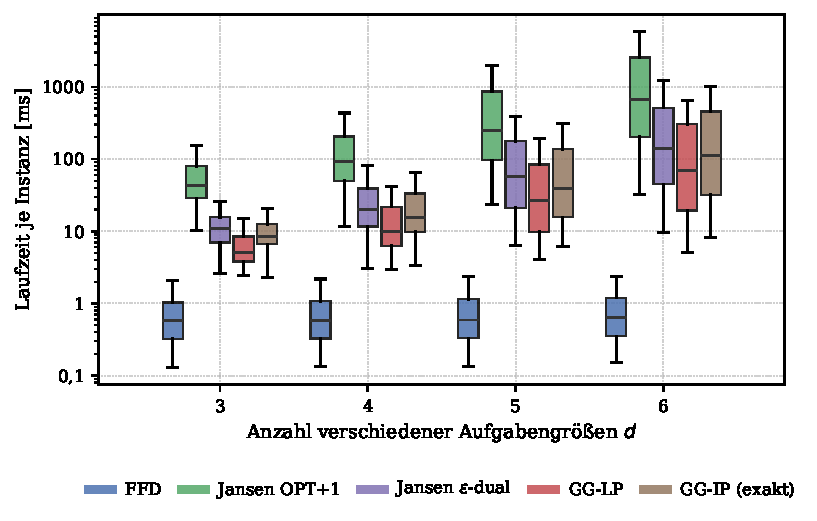
\includegraphics[width=0.94\textwidth]{figures/abb_hm_laufzeit.pdf}
\caption{Laufzeitverteilung je Subroutine über $d$ (logarithmische $y$-Achse, ohne Ausreißer).}
\label{fig:hm-laufzeit}
\end{figure}

Bemerkenswert ist die Reihenfolge: Das \emph{exakte} Konfigurationsprogramm
(\HmZeitMedianggip{}~ms) ist schneller als der $\mathrm{OPT}+1$-Algorithmus
(\HmZeitMedianjansen{}~ms).
Die Ursache ist die Zahl der Aufrufe des Lösers, nicht die Schwere der einzelnen Modelle.
Ein einzelnes MILP des $\mathrm{OPT}+1$-Algorithmus braucht im Median \HmMsProMilpJansen{}~ms und
damit kaum mehr als ein Konfigurationsprogramm mit \HmMsProModellGgip{}~ms.
Die innere Binärsuche nach $m^*$ löst davon je Kapazität jedoch \HmJansenMilpMedian{} Modelle im
Median und bis zu \HmJansenMilpMax, während das Konfigurationsprogramm mit einem auskommt.
Das Maximum ist genau die Schrittzahl einer Binärsuche über $\{1, \ldots, n\}$ bei
$n \le \HmNMax$, nämlich $\lfloor \log_2 \HmNMax \rfloor + 1 = \HmJansenMilpSchranke$.
Die $\varepsilon$-duale Variante, die diese Binärsuche durch die von außen bekannte
Maschinenzahl ersetzt (Abschnitt~\ref{sub:hm-aufbau}), liegt mit \HmZeitMedianjansendual{}~ms
dazwischen.

\subsection{Skalierung in der Multiplizität}
\label{sub:hm-skalierung}

Der Vorteil einer High-Multiplicity-Formulierung liegt darin, dass ihre Größe an der Anzahl $d$
verschiedener Größen hängt und nicht an der Anzahl $n$ der Aufgaben.
Für den $\mathrm{OPT}+1$-Algorithmus ist die Zahl der großen Konfigurationen bei festem $d$
konstant beschränkt (Abschnitt~\ref{sub:jansen-implementierung}).
Auf dem HM-Gitter mit $n \le \HmNMax$ ist das nicht messbar; dafür ist die HM-Skalierung
erzeugt worden.

Das Ergebnis trennt die Verfahren.
Während $n$ um den Faktor \HmSkalNFaktor{} wächst, steigt die Laufzeit von MULTIFIT+FFD um den
Faktor \HmSkalFaktorffd{} (Tabelle~\ref{tab:hm-skalierung}) - FFD verarbeitet jede Aufgabe
einzeln und läuft in $O(n \log n)$ (Abschnitt~\ref{sec:versuchsaufbau}).
Die vier High-Multiplicity-Subroutinen wachsen nur um das \HmSkalFaktorMin- bis
\HmSkalFaktorMax-fache.
Bei $n = \HmSkalNMax$ ist das Konfigurations-LP mit \HmSkalZeitMaxgglp{}~ms um ein Vielfaches
schneller als FFD mit \HmSkalZeitMaxffd{}~ms; der Schnittpunkt der beiden Medianverläufe liegt
nach log-linearer Interpolation zwischen den gemessenen Stützstellen bei etwa
$n \approx \HmSkalSchnittpunkt$ (Abbildung~\ref{fig:hm-skalierung}).

\begin{table}[htbp]
\centering
\small
\begin{tabular}{rrrrrrr}
\toprule
& & \multicolumn{5}{c}{Median der Laufzeit [ms]} \\
\cmidrule(lr){3-7}
$n$ & $m$ & FFD & Jansen OPT+1 & Jansen $\varepsilon$-dual & GG-LP & GG-IP (exakt) \\
\midrule
40 & 5 & 0{,}5 & 105{,}0 & 22{,}6 & 12{,}5 & 18{,}2 \\
400 & 50 & 5{,}7 & 416{,}9 & 55{,}9 & 22{,}7 & 37{,}0 \\
4\,000 & 500 & 79{,}9 & 372{,}7 & 46{,}6 & 23{,}9 & 33{,}8 \\
40\,000 & 5\,000 & 979{,}8 & 991{,}1 & 142{,}2 & 105{,}4 & 124{,}3 \\
\midrule
\multicolumn{2}{l}{Faktor} & 2\,118{,}2 & 9{,}4 & 6{,}3 & 8{,}5 & 6{,}8 \\
\bottomrule
\end{tabular}

\caption{Median der Laufzeit über die Multiplizitätsachse auf dem Datensatz HM-Skalierung,
  bei festem $d \in \{3,4\}$ und festem $n/m$. Die letzte Zeile gibt den Faktor zwischen der
  kleinsten und der größten Instanzgröße an; $n$ selbst wächst dabei um den Faktor
  \HmSkalNFaktor.}
\label{tab:hm-skalierung}
\end{table}

\begin{figure}[htbp]
\centering
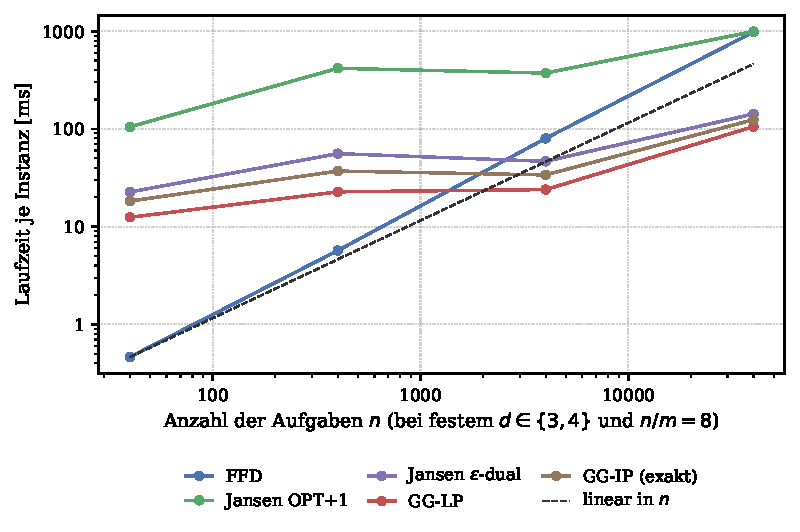
\includegraphics[width=0.92\textwidth]{figures/abb_hm_skalierung.pdf}
\caption{Laufzeit über $n$ bei festem $d \in \{3,4\}$ und festem $n/m$, doppelt logarithmisch.
  Die gestrichelte Linie wächst linear in $n$ und dient als Bezug.}
\label{fig:hm-skalierung}
\end{figure}

\subsection{Einschränkungen dieses Vergleichs}
\label{sub:hm-grenzen}

\begin{itemize}
  \item \textbf{Reichweite in $d$.} Alle Aussagen gelten für $d \le \HmDMax$. Die
    Konfigurationsmenge wächst mit $d$; auf den fünf Datensätzen aus
    Abschnitt~\ref{sec:benchmarks} liegt $d$ im Median zwischen \HmDBenchMedianMin{} und
    \HmDBenchMedianMax{} und damit außerhalb des Bereichs, für den
    Abschnitt~\ref{sub:anwendbarkeit} die Verfahren als sinnvoll ausweist. Gemessen wurden sie
    dort nicht.
  \item \textbf{Der additive Term.} Dass $\mathrm{GG}[\Gamma,C] - \mathrm{OPT}[\Gamma,C]$ hier
    \HmGGMaxUeberOpt{} nicht überschreitet, ist eine Aussage über diese Instanzen und kein Beleg
    gegen die Schranke $d-1$ aus Lemma~\ref{lem:gg-rundung}.
  \item \textbf{Zwei Instanzen mit abweichendem $d$.} In \HmDAbweichung{} Instanzen erzeugt der
    Generator eine Größe mit Vielfachheit null, sodass die Instanz weniger Typen enthält, als ihr
    Name angibt. Die Auswertung liest $d$ deshalb aus dem Instanzinhalt.
  \item \textbf{Laufzeitmessung.} Wie in Abschnitt~\ref{sec:grenzen}: eine Messung je Instanz,
    Mediane über Instanzen statt über Wiederholungen. Die Zeiten gelten für Gurobi in der
    beschriebenen Umgebung; ein anderer Löser verschiebt sie.
\end{itemize}
